\documentclass[border=3pt]{standalone}
\usepackage{helvet}
\renewcommand{\familydefault}{\sfdefault}
\usepackage[T1]{fontenc}
\usepackage{graphicx}
\usepackage{tikz}
\usepackage{amsmath}
\usetikzlibrary{arrows.meta,positioning,backgrounds,fit,calc}

\definecolor{stable}{RGB}{200,140,0}
\definecolor{unstable}{RGB}{197,27,125}
\definecolor{boxgray}{RGB}{244,244,244}
\definecolor{edge}{RGB}{90,90,90}
\definecolor{loadblue}{RGB}{70,110,160}

\newcommand{\panttl}[1]{{\footnotesize\bfseries #1}}

\begin{document}
\begin{tikzpicture}[font=\footnotesize]

% ---- overall two-row layout via coordinates ----
% TOP-LEFT: feedback schematic
\begin{scope}[shift={(0,0)},
  box/.style={draw=edge, rounded corners=1.5pt, fill=boxgray, align=center,
              minimum height=7.5mm, text width=27mm, inner sep=2.5pt},
  cbox/.style={draw=edge, rounded corners=1.5pt, align=center,
              minimum height=6.5mm, text width=20mm, inner sep=2pt},
  arr/.style={-{Latex[length=1.8mm]}, edge, line width=0.5pt}]

  \node[anchor=west] at (-0.2,3.05) {\panttl{a}\ \ \footnotesize\bfseries Cardiac G\&R as a feedback loop};

  \node[box, fill=loadblue!18] (load) at (1.6,2.35) {Hemodynamic load};
  \node[box, below=3.2mm of load] (dev) {Deviation from set-point $\Delta\sigma^i$};
  \node[cbox, fill=stable!22, below left=4mm and -12mm of dev] (myo) {Myocytes\\[-1pt]\scriptsize sarcomere turnover};
  \node[cbox, fill=unstable!14, below right=4mm and -12mm of dev] (col) {Collagen\\[-1pt]\scriptsize matrix turnover};
  \node[box, below=15mm of dev] (geo) {Adapted geometry \& mass};

  \draw[arr] (load) -- (dev);
  \draw[arr] (dev) -- (myo);
  \draw[arr] (dev) -- (col);
  \draw[arr] (myo) |- (geo);
  \draw[arr] (col) |- (geo);
  \draw[arr] (geo.west) -- ++(-5mm,0) |- (load.west);
  \node[edge, left=0mm of geo, xshift=-6mm, yshift=9mm, rotate=90] {\scriptsize feedback};
\end{scope}

% TOP-RIGHT: stable vs unstable hearts + colourbar
\begin{scope}[shift={(4.7,0)}]
  \node[anchor=west] at (0.0,3.05) {\panttl{b}\ \ \footnotesize\bfseries Predicted growth outcome};
  \node[anchor=north] (hs) at (1.25,2.65) {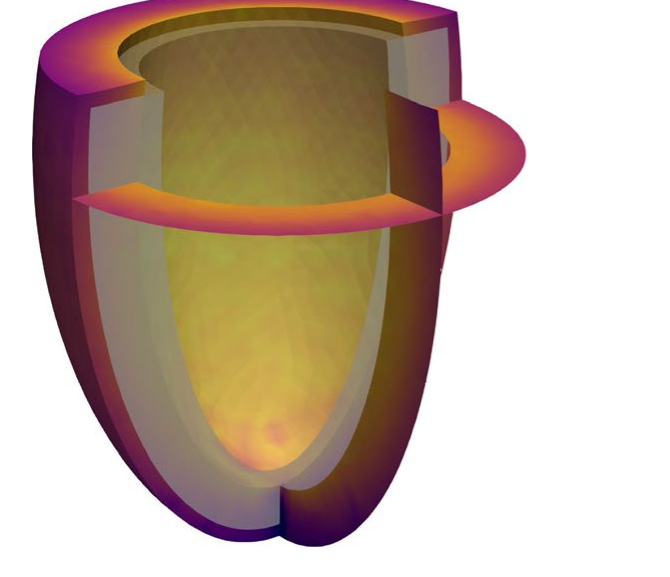
\includegraphics[width=2.7cm]{cut_stable_heart.png}};
  \node[stable, font=\scriptsize\bfseries, text width=2.9cm, align=center, anchor=north] at (hs.south){\textbf{Stable}\\[-1pt]\scriptsize returns to homeostasis};
  \node[anchor=north] (hu) at (4.15,2.72) {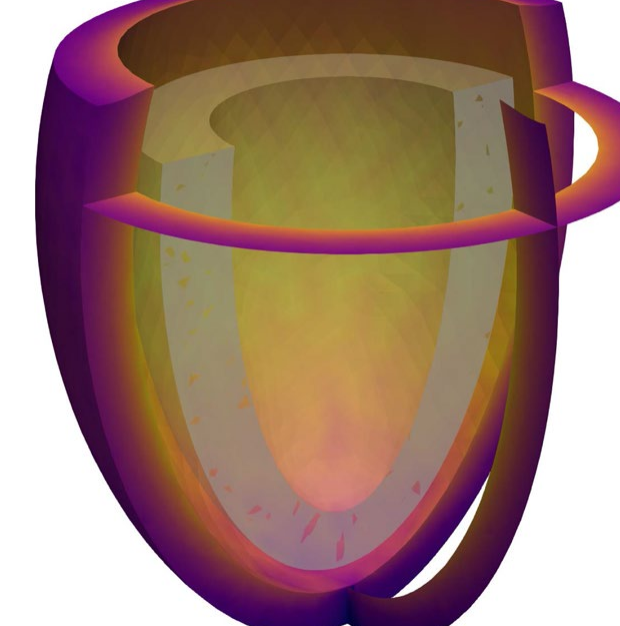
\includegraphics[width=2.7cm]{cut_unstable_heart.png}};
  \node[unstable, font=\scriptsize\bfseries, text width=2.9cm, align=center, anchor=north] at (hu.south){\textbf{Maladaptive}\\[-1pt]\scriptsize runaway dilation};
  \node[anchor=north] at (6.1,2.60) {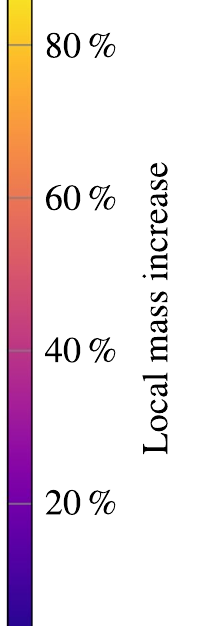
\includegraphics[height=2.55cm]{cut_massbar.png}};
\end{scope}

% BOTTOM: full-width time course
\begin{scope}[shift={(0,-3.05)}]
  \node[anchor=west] at (-0.2,0.30) {\panttl{c}\ \ \footnotesize\bfseries Remodeling time course: myocyte stress, wall thickness, chamber size, and collagen return to homeostasis (stable) or diverge (maladaptive)};
  \node[anchor=north west] at (0.0,-0.05) {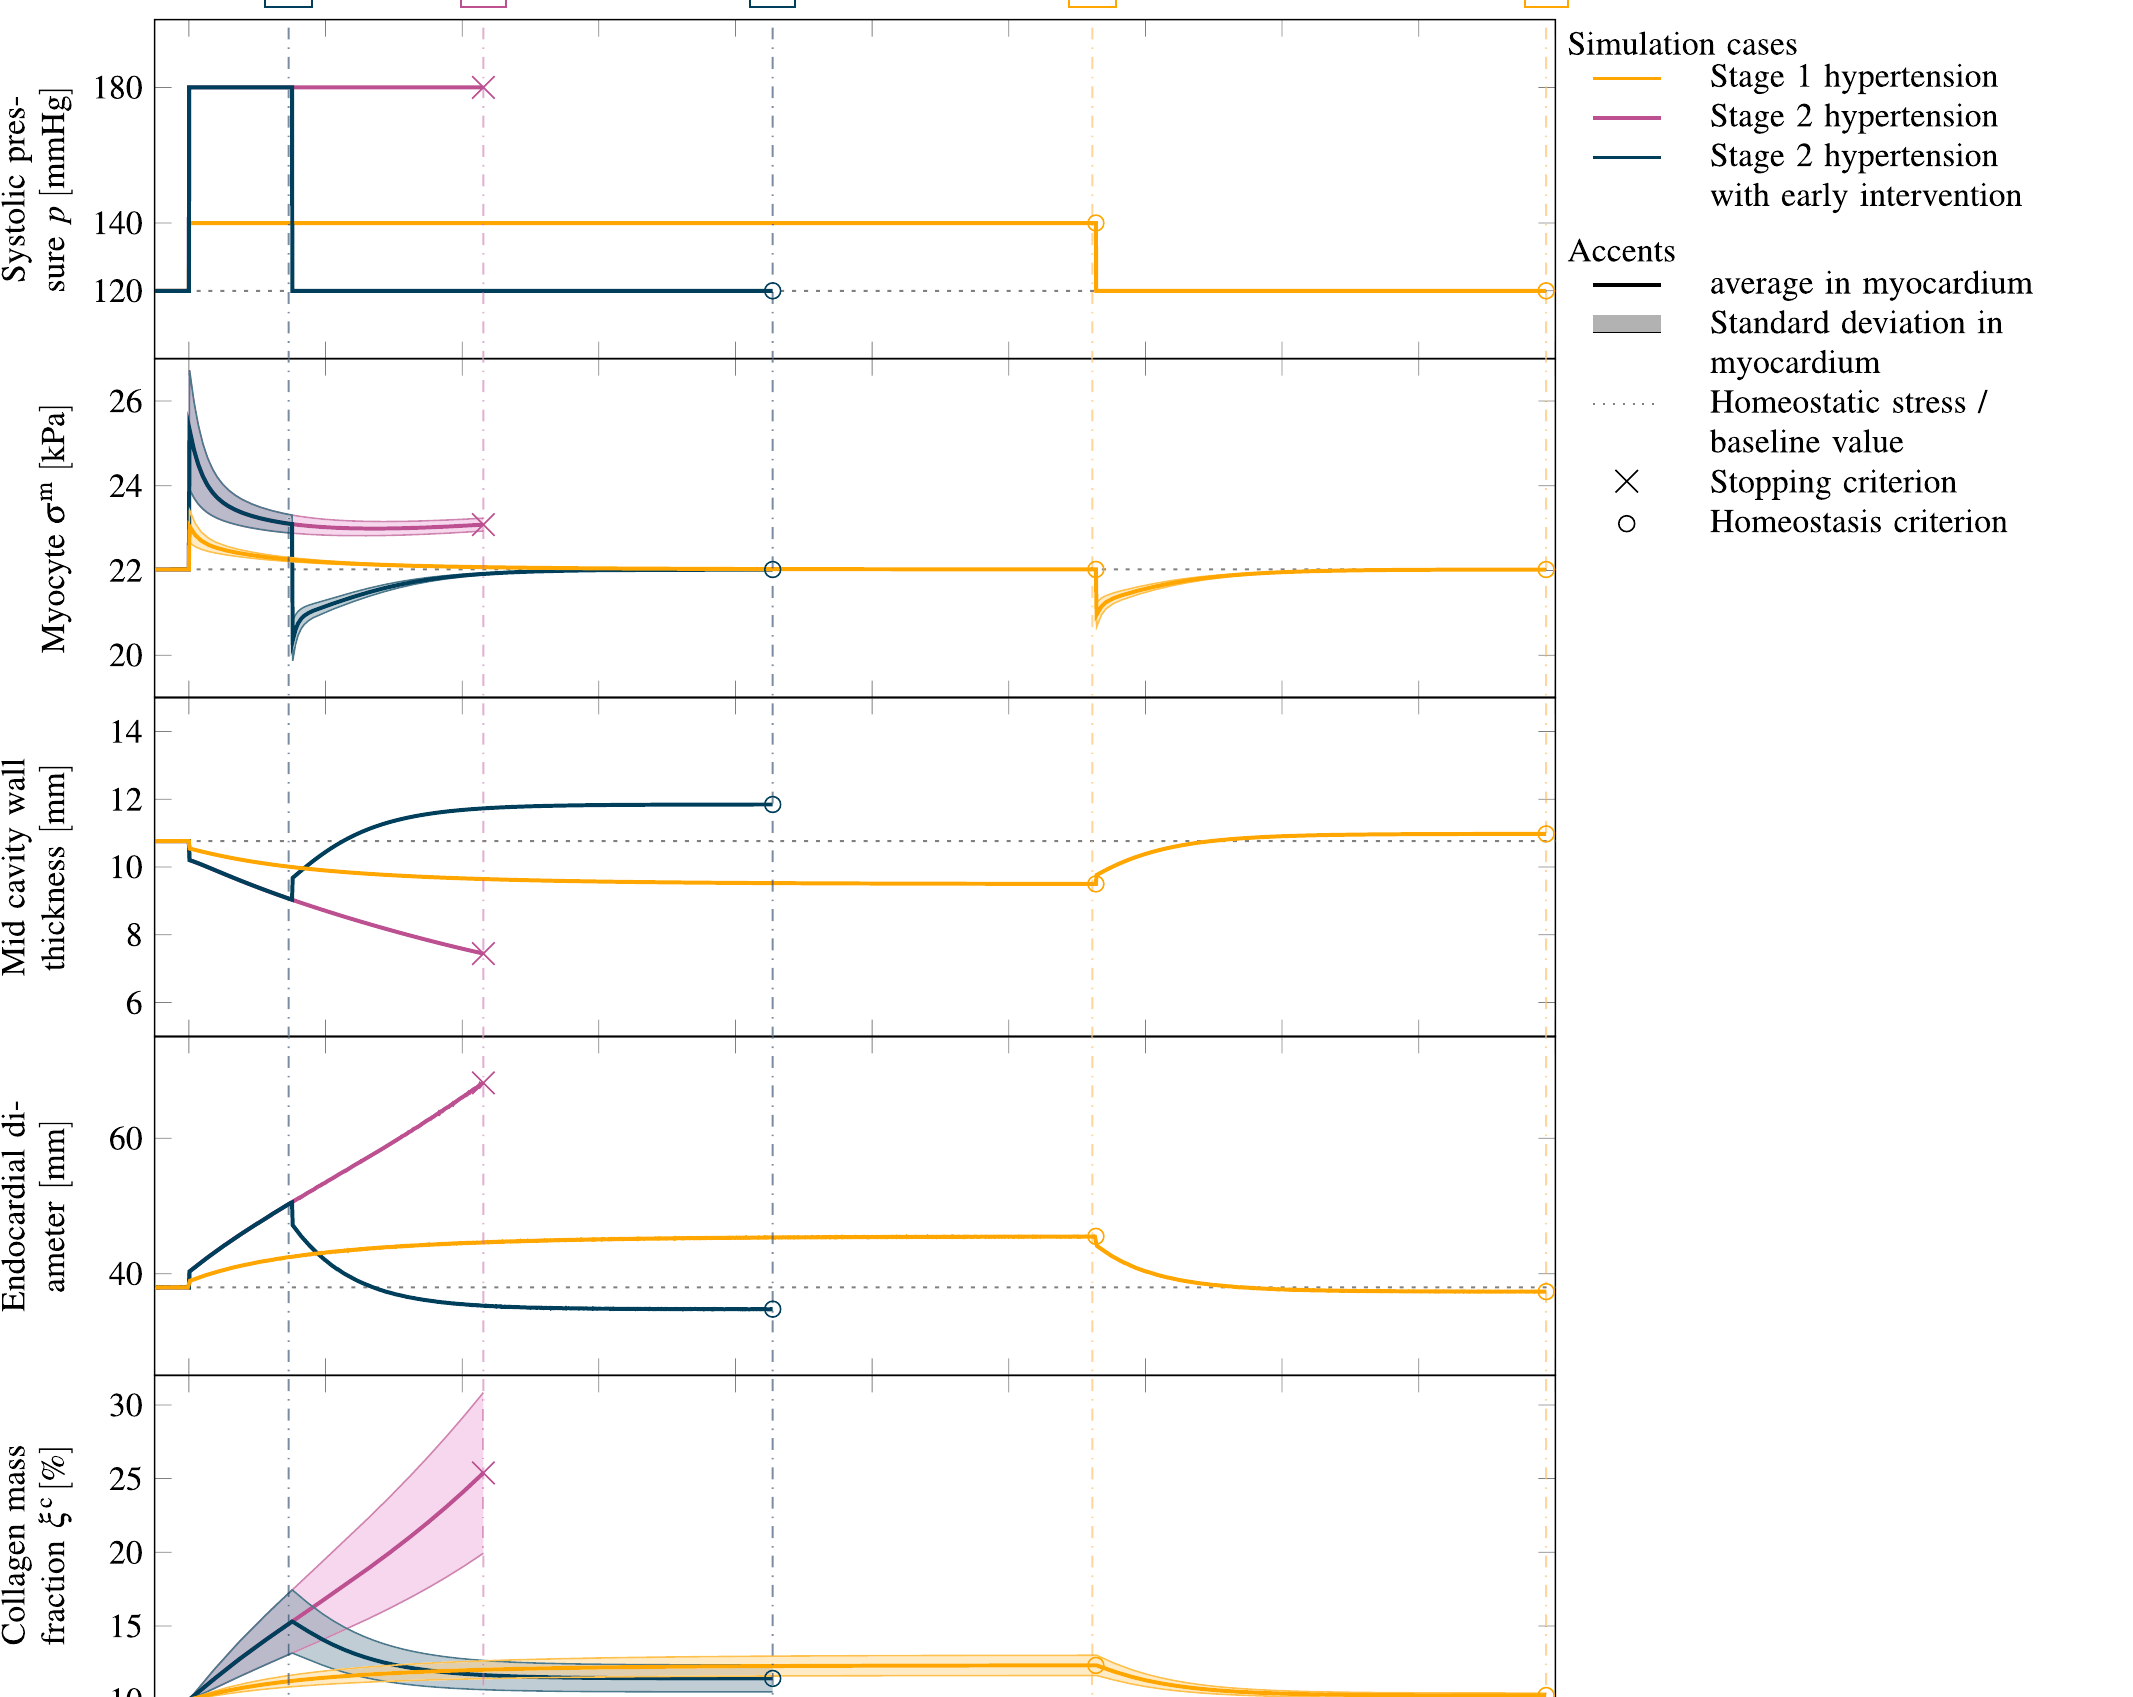
\includegraphics[width=11.9cm]{cut_timecourse.png}};
\end{scope}

\end{tikzpicture}
\end{document}
